% !TEX program = xelatex
% ============================================================
%  全国大学生数学建模竞赛 (CUMCM) LaTeX 通用论文模板
%  编译方式: XeLaTeX
% ============================================================
\documentclass[12pt,a4paper]{ctexart}

% ======================== 宏包加载 ========================
\usepackage[top=2.5cm, bottom=2.5cm, left=2.8cm, right=2.8cm]{geometry}
\usepackage{amsmath, amssymb, amsthm}
\usepackage{graphicx}
\usepackage{float}
\usepackage{subcaption}
\usepackage{booktabs}
\usepackage{array}
\usepackage{multirow}
\usepackage{longtable}
\usepackage{xcolor}
\usepackage{hyperref}
\hypersetup{
    colorlinks=true,
    linkcolor=blue!70!black,
    citecolor=green!50!black,
    urlcolor=blue!60!black
}
\usepackage{fvextra}
\DefineVerbatimEnvironment{CodeBlock}{Verbatim}{breaklines=true,fontsize=\small}

% ======================== 代码美化（附录用） ========================
\usepackage{listings}
\usepackage[most]{tcolorbox}

\lstdefinestyle{pystyle}{
  language=Python,
  basicstyle=\small\ttfamily,
  keywordstyle=\color{blue!70!black}\bfseries,
  commentstyle=\color{green!50!black}\itshape,
  stringstyle=\color{red!60!black},
  numbers=left,
  numberstyle=\tiny\color{gray},
  numbersep=6pt,
  backgroundcolor=\color{gray!5},
  breaklines=true,
  breakatwhitespace=true,
  tabsize=4,
  showstringspaces=false,
  captionpos=b,
  xleftmargin=1.5em,
  framexleftmargin=1.5em,
}

% 用法: \codefile{文件名}{说明}{相对路径}
\newcommand{\codefile}[3]{%
  \par\vspace{1.2em}\noindent
  \textbf{\texttt{#1}}\quad \textbf{#2}\par
  \vspace{0.4em}
  \lstinputlisting[style=pystyle]{#3}
  \vspace{0.5em}
}

\usepackage{setspace}
\usepackage{indentfirst}
\setlength{\parindent}{2em}
\onehalfspacing
\usepackage{enumitem}
\setlist{nosep, leftmargin=2em}
\usepackage{titlesec}
\usepackage{caption}
\usepackage{bm}
\usepackage{mathtools}
\usepackage{tikz}
\usetikzlibrary{trees}

% ======================== 图片路径 ========================
\graphicspath{{figures/}}

% ======================== 字体设置 ========================
\setCJKmainfont{SimSun}[BoldFont=SimHei, ItalicFont=KaiTi]
\setCJKsansfont{SimHei}
\setCJKmonofont{FangSong}
\setmainfont{Times New Roman}

% ======================== 编号格式 ========================
\renewcommand{\thesection}{\chinese{section}、}
\renewcommand{\thesubsection}{\arabic{section}.\arabic{subsection}}
\renewcommand{\thesubsubsection}{\arabic{section}.\arabic{subsection}.\arabic{subsubsection}}

% ======================== 标题格式 ========================
\titleformat{\section}
  {\centering\heiti\zihao{-3}\bfseries}
  {\thesection}{1em}{}
\titlespacing*{\section}{0pt}{1.5ex plus .5ex minus .2ex}{1.0ex plus .2ex}

\titleformat{\subsection}
  {\heiti\zihao{4}\bfseries}
  {\thesubsection}{1em}{}
\titlespacing*{\subsection}{0pt}{1.2ex plus .4ex minus .2ex}{0.8ex plus .2ex}

\titleformat{\subsubsection}
  {\heiti\zihao{-4}\bfseries}
  {\thesubsubsection}{1em}{}
\titlespacing*{\subsubsection}{0pt}{1.0ex plus .3ex minus .1ex}{0.6ex plus .1ex}

% ======================== 定理环境 ========================
\theoremstyle{definition}
\newtheorem{definition}{定义}[section]
\newtheorem{assumption}{假设}[section]
\theoremstyle{plain}
\newtheorem{theorem}{定理}[section]
\newtheorem{lemma}{引理}[section]
\newtheorem{proposition}{命题}[section]
\newtheorem{corollary}{推论}[section]
\theoremstyle{remark}
\newtheorem{remark}{注}[section]

% ======================== 自定义命令 ========================
\renewenvironment{abstract}
  {\begin{center}\heiti\zihao{-3}摘\quad 要\end{center}\zihao{-4}\songti}
  {\par\vspace{1em}}

\newcommand{\keywords}[1]{%
  \par\noindent\textbf{关键词：}#1}

\newenvironment{symboltable}
  {\begin{center}\zihao{5}\begin{tabular}{>{\centering\arraybackslash}p{3.5cm} p{7.5cm} >{\centering\arraybackslash}p{1.5cm}}
  \toprule
  \textbf{符号} & \textbf{含义} & \textbf{单位} \\
  \midrule}
  {\bottomrule\end{tabular}\end{center}}

\newcommand{\step}[1]{\par\noindent\textbf{Step #1}\quad}

% ============================================================
\begin{document}
\pagestyle{plain}

\begin{center}
{\zihao{-2}\heiti\bfseries 基于综合评价方法和时间序列模型的原材料订购问题研究}
\end{center}
\vspace{1em}

% ======================== 摘要 ========================
\setcounter{page}{1}
\pagenumbering{arabic}

\begin{abstract}
  
为保障生产企业持续稳定发展，针对生产企业原材料订购与供应问题，本文建立了CRITIC及TOPSIS综合评价模型帮助企业筛选高质量合作供应商，并根据企业生产需求建立0-1整数规划模型和并利用偏差序列ARIMA模型对供应商未来供货情况进行预测，以此制定企业未来24周的订购计划及供货商的供货计划。

{\heiti 针对问题一：}本文首先对402家供应商近5年共240周的订货量与供货量历史数据进行量化分析。通过研究数据分布特性，识别出供货规模、缺货缺口、履约可靠性和波动幅度四个关键评价维度，并据此构建特征指标体系。在此基础上，采用 \textbf{CRITIC-TOPSIS} 法客观赋权与综合评价，最终筛选出55家最重要供应商。结果显示供货达标率权重最高，体现了模型对履约可靠性的重视。经熵权法交叉验证，两种方法排名高度一致，证明评价结果具有稳健性。

{\heiti 针对问题二：}在问题一基础上，以每周是否向供应商订货为决策变量，以最小化采购总成本为目标建立\textbf{0-1整数规划模型}。约束条件包括每周总订购量折算产品体积不低于产能百分之九十，以及各供应商订货次数不低于历史平均周期订货次数。求解得到未来24周最优订购方案，所有周次均满足产能底线要求。

{\heiti 针对问题三：}构建每家供应商的供货偏差序列，通过ADF检验和Ljung-Box检验判断序列特性，分别采用\textbf{ARIMA模型}或均值模型预测未来24周偏差。将预测偏差叠加固定订货量得到实际供货量预测值。计算得出平均产能满足率为101.31\%，达标周数占比\textbf{91.7\%}。蒙特卡洛模拟显示每周达标概率为92.12\%，方案具有较高可靠性。
\end{abstract}

\keywords{CRITIC赋权；TOPSIS排序；0-1整数规划；偏差序列ARIMA}

\newpage

% ============================================================
%  正文
% ============================================================

\section{问题重述}

\subsection{问题背景}

某建筑和装饰板材生产企业的主要原材料为木质纤维及其他植物素纤维材料，总体分为A、B、C三种类型。该企业每年按两个周期（共计48周）安排生产，需要提前制定一个周期（24周）的原材料订购与转运计划，即根据产能要求确定需要订购的原材料供应商以及相应的每周原材料订购数量。

该企业每周产能为2.82万立方米，每生产一立方米产品需消耗A类原材料0.6立方米，或B类原材料0.66立方米，或C类原材料0.72立方米。由于原材料自身的特殊性，供应商无法保证严格按订货量供货，实际供货量可能多于或少于订货量，因此该企业对供应商实际提供的原材料总是全部收购。实际中，A类和B类原材料的采购单价分别比C类原材料高20\%和10\%。

\subsection{问题提出}

附件1提供了该企业近5年402家原材料供应商的订货量和供货量数据。我们应结合实际情况，对相关数据进行深入分析，研究下列问题：

问题一：根据附件1，对402家供应商的订货和供货特征进行量化分析，建立能够反映保障企业生产重要性的数学模型，并在此基础上确定55家最重要的供应商。

问题二：针对问题1选出的55家供应商，经企业与供应商协商后，企业以每个供应商过去的每周平均订货量作为订货量，且订货次数必须大于或等于该供应商的平均周期订货次数，同时要求每周的总订购量至少达到产能的90\%以上。为该企业制定这些供应商未来24周每周最优的原材料订购方案，该方案需明确每一周向哪些供应商进行订购。

问题三：在问题2结果的基础上，根据供应商的供货特征，为这些供应商制定未来24周每周的原材料供应方案，并统计达到周产能需求的比例。

\section{问题分析}

\subsection{问题一的分析}

本题要求从402家供应商中筛选出55家最重要的供应商，属于多属性综合评价问题。题目提供了近5年240周的订货量和供货量数据，但未明确评价指标体系，需要自行设计特征。关键难点在于如何量化保障企业生产的重要性。我们从供应链管理角度出发，设计四个评价维度：供货能力即周供货量均值，履约质量即周供货缺失量均值，供货达标率即供货量不低于订货量的周数占比，以及供货稳定性即供货量与订货量差值的均方差。这些指标能够全面反映供应商对企业生产的保障程度。评价方法采用CRITIC权重法确定各指标客观权重，结合TOPSIS法进行供应商优劣排序，确保评价结果的科学性和客观性。

\subsection{问题二的分析}

本题要求为筛选出的55家供应商制定未来24周的最优订购方案。题目给出的关键约束包括：每周总订购量需达到产能的百分之九十以上，订货次数需大于等于平均周期订货次数，且以历史平均订货量四舍五入取整为订货量。核心难点是建立0-1整数规划模型，在满足产能保障和订货频次两个硬约束的前提下，实现采购总成本最小化。

\subsection{问题三的分析}

本题要求根据供应商历史供货特征制定未来24周的供货方案，本质上是一个回归预测问题。关键信息是供货量与订货量之间存在动态关系：当周订货量增大会占用供应商供货能力，导致下周供货量相对降低，反之则提高。同时，订货量对供货量具有锚定作用，供货量会在订货量附近波动。因此，对供货量的预测必须嵌入订货量信息，采用时间序列模型对每周订货量与实际供货量的差值进行预测。选择时间序列模型而非简单线性回归的原因在于：供货量数据具有明显的时序依赖性，当前周的供货量受前几周订货量的累积影响，线性回归无法捕捉这种动态滞后效应；订货量与供货量差值可能存在趋势性和周期性特征，ARIMA模型通过差分和自回归项能够有效识别并建模这些时序模式；线性回归假设样本独立同分布，而时间序列数据存在自相关性，使用线性回归会导致参数估计偏误和预测区间失真。ARIMA模型能够充分利用历史信息的时序结构，提供更准确的预测结果。

\section{模型假设}

\begin{enumerate}[label=\arabic*.]
  \item 假设未来24周各供应商的供货偏差规律与历史保持一致。
  \item 假设三类原材料的单位消耗系数在未来保持恒定，不随批次或季节波动。
  \item 假设数据中的零值均代表未发生实际业务往来或当周供货缺失。
\end{enumerate}


\section{符号说明}

\begin{symboltable}
$O_{ij}$ & 第i家供应商第j周的订货量 & 立方米 \\
$S_{ij}$ & 第i家供应商第j周的实际供货量 & 立方米 \\
$W_i$ & 第i家供应商的有效订货周集合 & 无 \\
$N_i$ & 第i家供应商的有效订货周数 & 周 \\
$Q_i$ & 第i家供应商的固定订货量 & 立方米 \\
$D_{ij}$ & 第i家供应商第j周的供货偏差 & 立方米 \\
$u_i$ & 第i家供应商所供材料的单位产品消耗率 & 立方米每立方米 \\
$x_{ij}$ & 第j周是否向第i家供应商订货 & 无 \\
$p_i$ & 第i家供应商的采购单价 & 无 \\
$K_i$ & 第i家供应商的最低订货次数 & 次 \\
$C_i$ & 第i家供应商的贴近度 & 无 \\
\end{symboltable}


\section{模型建立与求解}

\subsection{数据预处理}

\subsubsection{原始数据说明}

附件1包含两个工作表："企业的订货量"和"供应商的供货量"，每张表均为$409$行$\times 242$列结构。前两列为供应商ID（S001--S402）和材料分类（A/B/C），第3至242列为W001至W240共240周的订货量或供货量数据，单位为立方米。

\subsubsection{缺失值与异常值处理}

对原始数据进行如下预处理：

（1）剔除表头行与可能的空行，保留402家供应商的有效记录。

（2）对订货量表与供货量表按供应商ID对齐，确保同一供应商的订货数据与供货数据一一对应。

（3）将缺失值统一填充为0。在本题语境下，订货量为0表示该周未向该供应商下单，供货量为0表示该周该供应商未供货，0值具有明确实际含义并非单纯的缺失。

（4）检查是否存在240周内从未被订过货的供应商，若存在则其有效周数$N_i = 0$，无法计算统计特征，予以剔除。实际数据中402家供应商均有订货记录，无需剔除。

\subsubsection{有效订货周界定}

为规避企业和供应商未发生业务往来的周次（$O_{ij} = 0$）对均值、方差等统计量的稀释干扰，定义第$i$家供应商的有效订货周集合：

\begin{equation}
W_i = \{j \mid O_{ij} > 0\}, \quad i = 1, 2, \dots, 402
\end{equation}

其有效周数记为$N_i = |W_i|$。后续所有特征指标的计算均在$W_i$上进行。

\subsection{问题一模型建立及求解}

\subsubsection{建模前准备}


根据问题一的分析，评价指标应能刻画供应商的供货特征，反映其对保障企业生产的重要性。本文遵循系统性、科学性、可比性和可测性四个原则选取指标。基于上述原则，本文构建如图\ref{fig:framework}所示的评价指标框架。

\begin{figure}[H]
\centering
\begin{tikzpicture}[
  level 1/.style={sibling distance=58mm, level distance=18mm},
  level 2/.style={sibling distance=28mm, level distance=18mm},
  every node/.style={draw, rectangle, align=center, font=\small, text width=20mm, minimum height=6mm}
]
\node {供应商重要性}
  child {node {供货能力}
    child {node {$F_1$\\周均供货量}}
    child {node {$F_2$\\周均缺失量}}
  }
  child {node {履约可靠性}
    child {node {$F_3$\\供货达标率}}
    child {node {$F_4$\\偏差均方}}
  };
\end{tikzpicture}
\caption{问题一评价指标框架}
\label{fig:framework}
\end{figure}

\subsubsection{特征指标提取}

针对第$i$家供应商，从供货规模、信用缺口、履约可靠性、供货波动四个维度提取评价指标。

\textbf{1. 周均供货量$F_{1i}$}

第$i$家供应商的周均供货量定义为该供应商在有效订货周上供货量的算术平均：

\begin{equation}
F_{1i} = \frac{1}{N_i} \sum_{j \in W_i} S_{ij}, \quad i = 1, 2, \dots, 402
\end{equation}

其中$S_{ij}$为第$i$家供应商第$j$周的实际供货量。$F_{1i}$为极大型指标，其值越大，表明该供应商的平均周产能贡献越高，在保障企业连续生产方面的规模优势越显著。

\textbf{2. 周均供货缺失量$F_{2i}$}

第$i$家供应商的周均供货缺失量定义为该供应商在有效订货周上订货量超出供货量部分（即缺货缺口）的算术平均：

\begin{equation}
F_{2i} = \frac{1}{N_i} \sum_{j \in W_i} \max(0,\; O_{ij} - S_{ij}), \quad i = 1, 2, \dots, 402
\end{equation}

其中$O_{ij}$为第$i$家供应商第$j$周的订货量。$F_{2i}$为极小型指标，引入截断函数$\max(\cdot, 0)$仅统计缺货方向的差值，防止超额供货的冗余量抵消缺货量。其值越小，表明该供应商的履约信用越好，订货缺口越可控。

\textbf{3. 供货达标率$F_{3i}$}

第$i$家供应商的供货达标率定义为该供应商在有效订货周上供货量不低于订货量的周次占比：

\begin{equation}
F_{3i} = \frac{1}{N_i} \sum_{j \in W_i} I(S_{ij} \geq O_{ij}), \quad i = 1, 2, \dots, 402
\end{equation}

其中$I(\cdot)$为指示函数，条件成立取1，否则取0。$F_{3i}$为极大型指标，采用$\geq$（含等号）使精确交货（$S_{ij} = O_{ij}$）计入达标，度量的是"履约可靠性"而非"超额供货倾向"。其值越接近1，表明该供应商连续稳定供货的能力越强。

\textbf{4. 供货均方偏差$F_{4i}$}

第$i$家供应商的供货偏差均方定义为该供应商在有效订货周上订货量与供货量偏差平方的算术平均：

\begin{equation}
F_{4i} = \frac{1}{N_i} \sum_{j \in W_i} (O_{ij} - S_{ij})^2, \quad i = 1, 2, \dots, 402
\end{equation}

$F_{4i}$为极小型指标，反映供货偏差的离散程度。其值越小，表明该供应商供货波动越平缓，可靠性越高；其值越大，表明供货量围绕订货量剧烈震荡，企业难以据此安排稳定生产。

上述四项指标从规模、信用、可靠性、稳定性四个互补维度刻画供应商的综合特征，构成后续CRITIC赋权与TOPSIS排序的原始特征矩阵$X = (x_{ik})_{402 \times 4}$，其中$k = 1, 2, 3, 4$分别对应$F_1$、$F_2$、$F_3$、$F_4$。

\subsubsection{模型求解}


（1）CRITIC客观赋权流程如下：

\textbf{Step 1：数据正向化与标准化}

为消除指标量纲与方向差异，对极大型指标（$F_1$、$F_3$）和极小型指标（$F_2$、$F_4$）分别进行min-max标准化。

\begin{equation}
y_{ik} = 
\begin{cases}
\dfrac{x_{ik} - \min_i(x_{ik})}{\max_i(x_{ik}) - \min_i(x_{ik})}, & \text{极大型指标} \\[10pt]
\dfrac{\max_i(x_{ik}) - x_{ik}}{\max_i(x_{ik}) - \min_i(x_{ik})}, & \text{极小型指标}
\end{cases}
\end{equation}

标准化后所有指标取值落于$[0, 1]$区间，且方向统一为"越大越优"，得到标准化矩阵$Y = (y_{ik})_{402 \times 4}$。

\textbf{Step 2：计算对比强度}

对标准化矩阵$Y$，计算第$k$项指标的样本标准差作为对比强度：

\begin{equation}
\sigma_k = \sqrt{\frac{1}{402-1} \sum_{i=1}^{402} (y_{ik} - \bar{y}_k)^2}, \quad k = 1, 2, 3, 4
\end{equation}

其中$\bar{y}_k$为第$k$项指标的样本均值。$\sigma_k$越大，说明该指标在402家供应商间的离散程度越高，区分能力越强。

\textbf{Step 3：计算指标冲突性}

计算指标间的Pearson相关系数矩阵$R = (r_{jk})_{4 \times 4}$：

\begin{equation}
r_{jk} = \frac{\sum_{i=1}^{402}(y_{ij} - \bar{y}_j)(y_{ik} - \bar{y}_k)}{\sqrt{\sum_{i=1}^{402}(y_{ij} - \bar{y}_j)^2 \sum_{i=1}^{402}(y_{ik} - \bar{y}_k)^2}}
\end{equation}

第$k$项指标的冲突性定义为：

\begin{equation}
\gamma_k = \sum_{j=1}^{4} (1 - r_{jk}), \quad k = 1, 2, 3, 4
\end{equation}

$r_{jk}$越接近1，两指标信息越冗余，冲突性越小；$r_{jk}$越接近0或为负，独立信息越多，冲突性越大。

\textbf{Step 4：计算综合权重}

第$k$项指标的信息承载量为对比强度与冲突性的乘积：

\begin{equation}
I_k = \sigma_k \cdot \gamma_k
\end{equation}

归一化得最终权重：

\begin{equation}
w_k = \frac{I_k}{\sum_{k=1}^{4} I_k}, \quad k = 1, 2, 3, 4
\end{equation}

（2）TOPSIS综合排序流程如下：

\textbf{Step 1：构建加权标准化矩阵}

利用CRITIC权重$w_k$对标准化矩阵$Y$逐列加权，得到加权标准化矩阵$Z = (z_{ik})_{402 \times 4}$：

\begin{equation}
z_{ik} = w_k \cdot y_{ik}, \quad i = 1, 2, \dots, 402;\; k = 1, 2, 3, 4
\end{equation}

加权后的矩阵既保留了各指标的标准化得分，又体现了CRITIC赋予的相对重要性。

\textbf{Step 2：确定正理想解与负理想解}

正理想解$Z^+$取各列最大值，负理想解$Z^-$取各列最小值：

\begin{equation}
Z_k^+ = \max_i(z_{ik}), \quad Z_k^- = \min_i(z_{ik}), \quad k = 1, 2, 3, 4
\end{equation}

正理想解代表所有供应商在各指标上的最优表现组合，负理想解代表最差表现组合。

\textbf{Step 3：计算欧氏距离}

各供应商到正、负理想解的欧氏距离分别为：

\begin{equation}
\begin{cases}
D_i^+ = \sqrt{\sum_{k=1}^{4} (z_{ik} - Z_k^+)^2} \\[10pt]
D_i^- = \sqrt{\sum_{k=1}^{4} (z_{ik} - Z_k^-)^2}
\end{cases}
\quad i = 1, 2, \dots, 402
\end{equation}

$D_i^+$越小，表明该供应商越接近最优表现；$D_i^-$越大，表明该供应商越远离最差表现。

\textbf{Step 4：计算相对贴近度}

第$i$家供应商的相对贴近度定义为：

\begin{equation}
C_i = \frac{D_i^-}{D_i^+ + D_i^-}, \quad i = 1, 2, \dots, 402
\end{equation}

$C_i \in [0, 1]$，越接近1表示该供应商越接近正理想解、远离负理想解，综合表现越优。


\subsubsection{结果展示}

\begin{table}[H]
\centering
\caption{CRITIC权重分析结果}
\label{tab:critic}
\zihao{5}
\begin{tabular}{cccc}
\toprule
指标 & CRITIC权重 & 对比强度 & 冲突性 \\
\midrule
周均供货量 & 0.2847 & 0.1213 & 3.4661 \\
周均缺失量 & 0.0922 & 0.0564 & 2.4139 \\
供货达标率 & 0.5325 & 0.2927 & 2.6872 \\
供货偏差均方 & 0.0907 & 0.0533 & 2.5144 \\
\bottomrule
\end{tabular}
\end{table}
CRITIC法中供货达标率权重最高，说明在保障企业生产重要性方面，履约可靠性比供货规模更具区分价值。

最终通过CRITIC赋权并借助TOPSIS法计算综合得分并排名，得出的最重要的55家供应商汇成表格如下。

\begin{table}[H]
\centering
\caption{最重要的55家供应商及其贴近度}
\label{tab:top55}
\begin{tabular}{ccccccccc}
\toprule
供应商ID & 贴近度 & 供应商ID & 贴近度 & 供应商ID & 贴近度 \\
\midrule
S229 & 0.9521 & S352 & 0.7044 & S239 & 0.6537 \\
S361 & 0.9166 & S348 & 0.7014 & S342 & 0.6531 \\
S108 & 0.8477 & S143 & 0.6937 & S379 & 0.6527 \\
S140 & 0.8404 & S037 & 0.6911 & S055 & 0.6523 \\
S282 & 0.7968 & S374 & 0.6877 & S294 & 0.6520 \\
S340 & 0.7812 & S247 & 0.6860 & S175 & 0.6518 \\
S151 & 0.7775 & S284 & 0.6851 & S221 & 0.6510 \\
S275 & 0.7701 & S126 & 0.6836 & S080 & 0.6508 \\
S329 & 0.7672 & S365 & 0.6735 & S237 & 0.6506 \\
S395 & 0.7664 & S031 & 0.6701 & S367 & 0.6504 \\
S139 & 0.7587 & S338 & 0.6662 & S213 & 0.6480 \\
S356 & 0.7494 & S364 & 0.6605 & S114 & 0.6479 \\
S131 & 0.7459 & S178 & 0.6586 & S005 & 0.6472 \\
S268 & 0.7441 & S053 & 0.6584 & S244 & 0.6471 \\
S330 & 0.7438 & S218 & 0.6578 & S346 & 0.6470 \\
S308 & 0.7403 & S067 & 0.6569 & S169 & 0.6465 \\
S306 & 0.7400 & S174 & 0.6567 & S076 & 0.6460 \\
S194 & 0.7210 & S040 & 0.6552 &  &  &  \\
S307 & 0.7091 & S362 & 0.6550 &  &  &  \\
\bottomrule
\end{tabular}
\end{table}

\subsection{问题二模型建立及求解}

\subsubsection{目标函数确定}

在问题一筛选出的55家核心供应商基础上，企业需要制定未来24周的原材料订购方案。每次向某家供应商发出订单时，订购量固定为该供应商的历史周均订货量并取整，企业只需决定每周是否向该供应商下单。这是一个典型的0-1选择问题。

三种材料类型的采购单价存在差异：A类为C类的1.2倍，B类为1.1倍。但将单价与消耗率结合后，A类与C类的单位产品成本精确相等（均为0.720），B类仅高出0.83\%。因此，成本目标对A类和C类供应商完全无差异，模型在两者之间的选择将由产能约束和频次约束而非成本驱动。

以每周是否向供应商订货为决策变量：
\begin{equation}
x_{ij} \in \{0, 1\}, \quad i = 1, 2, \dots, 55;\; j = 1, 2, \dots, 24
\label{eq:decision2}
\end{equation}
$x_{ij}=1$表示第$j$周向第$i$家供应商订货。每家供应商的固定订货量$Q_i$取历史有效周均订货量并取整：
\begin{equation}
Q_i = \text{round}\!\left(\frac{1}{N_i}\sum_{j \in W_i} O_{ij}\right)
\label{eq:qi2}
\end{equation}
$Q_i$的范围从1到1261立方米不等。以最小化24周采购总成本为目标：
\begin{equation}
\min Z = \sum_{j=1}^{24} \sum_{i=1}^{55} p_i \cdot Q_i \cdot x_{ij}
\label{eq:objective2}
\end{equation}

\subsubsection{约束条件}

\textbf{Step 1：周产能底线约束}

企业周产能为28200立方米，为保障生产连续性，每周订购量折算为产品体积后不得低于产能的百分之九十。$Q_i$为原材料体积，需按消耗率$u_i$折算，A类0.6，B类0.66，C类0.72。
\begin{equation}
\sum_{i=1}^{55} \frac{Q_i}{u_i} \cdot x_{ij} \geq 25380, \quad \forall\, j \in \{1, 2, \dots, 24\}
\label{eq:capacity2}
\end{equation}
55家全选时的周产能为26176立方米，仅超出底线百分之3.1，说明这是一个产能余量极薄的紧约束问题。

\textbf{Step 2：最低订购频次约束}

维持稳定的供销关系需要每家供应商的订货次数不低于其历史平均周期订货次数。$K_i$取过去240周中该供应商有订货记录的周数除以10后向上取整：
\begin{equation}
K_i = \lceil \frac{1}{10} \sum_{j=1}^{240} I(O_{ij} > 0) \rceil
\label{eq:fi2}
\end{equation}
$K_i$范围从4到24次，总和为1081次。此约束确保模型不会因成本最小化而完全放弃与某些供应商的合作。
\begin{equation}
\sum_{j=1}^{24} x_{ij} \geq K_i, \quad \forall\, i \in \{1, 2, \dots, 55\}
\label{eq:frequency2}
\end{equation}

\subsubsection{模型汇总}

综合目标函数与约束条件，问题二的0-1整数线性规划模型归纳如下：
\begin{align*}
&\min \; Z = \sum_{j=1}^{24} \sum_{i=1}^{55} p_i \cdot Q_i \cdot x_{ij} \\
\text{s.t.} \quad
&\sum_{i=1}^{55} \frac{Q_i}{u_i} \cdot x_{ij} \geq 25380, \quad j = 1, \dots, 24 \\
&\sum_{j=1}^{24} x_{ij} \geq K_i, \quad i = 1, \dots, 55 \\
&x_{ij} \in \{0, 1\}, \quad \forall\, i, j
\end{align*}
目标为在产能保障和供销关系维持的双重约束下实现采购总成本最小化。

\subsubsection{模型求解}

采用\textbf{分支定界法}求解上述0-1整数线性规划，求解器选用PuLP调用CBC求解器，适合该中小规模整数规划问题。

\textbf{模型规模：}共1320个0-1决策变量，24个产能约束与55个频次约束，合计79个线性约束。

\textbf{求解状态：}Optimal（全局最优解）。

\textbf{求解效率：}求解时间为秒级，表明模型规模适中、约束结构良好。

\textbf{最优目标值：}24周总采购成本为445935.30。

\subsubsection{结果展示}

\begin{table}[H]
\centering
\caption{问题二订购方案统计结果}
\label{tab:order}
\zihao{5}
\begin{tabular}{cc}
\toprule
指标 & 数值 \\
\midrule
求解状态 & Optimal（全局最优） \\
24周总成本 & 445935.30 \\
平均周订购量 & 25733 立方米 \\
最小周订购量 & 25381 立方米 \\
最大周订购量 & 26067 立方米 \\
达标周数 & 24周全部达标 \\
平均每周供应商数 & 46.8 家 \\
\bottomrule
\end{tabular}
\end{table}

图\ref{fig:volume}展示了24周订购量的变化情况。
\begin{figure}[H]
\centering
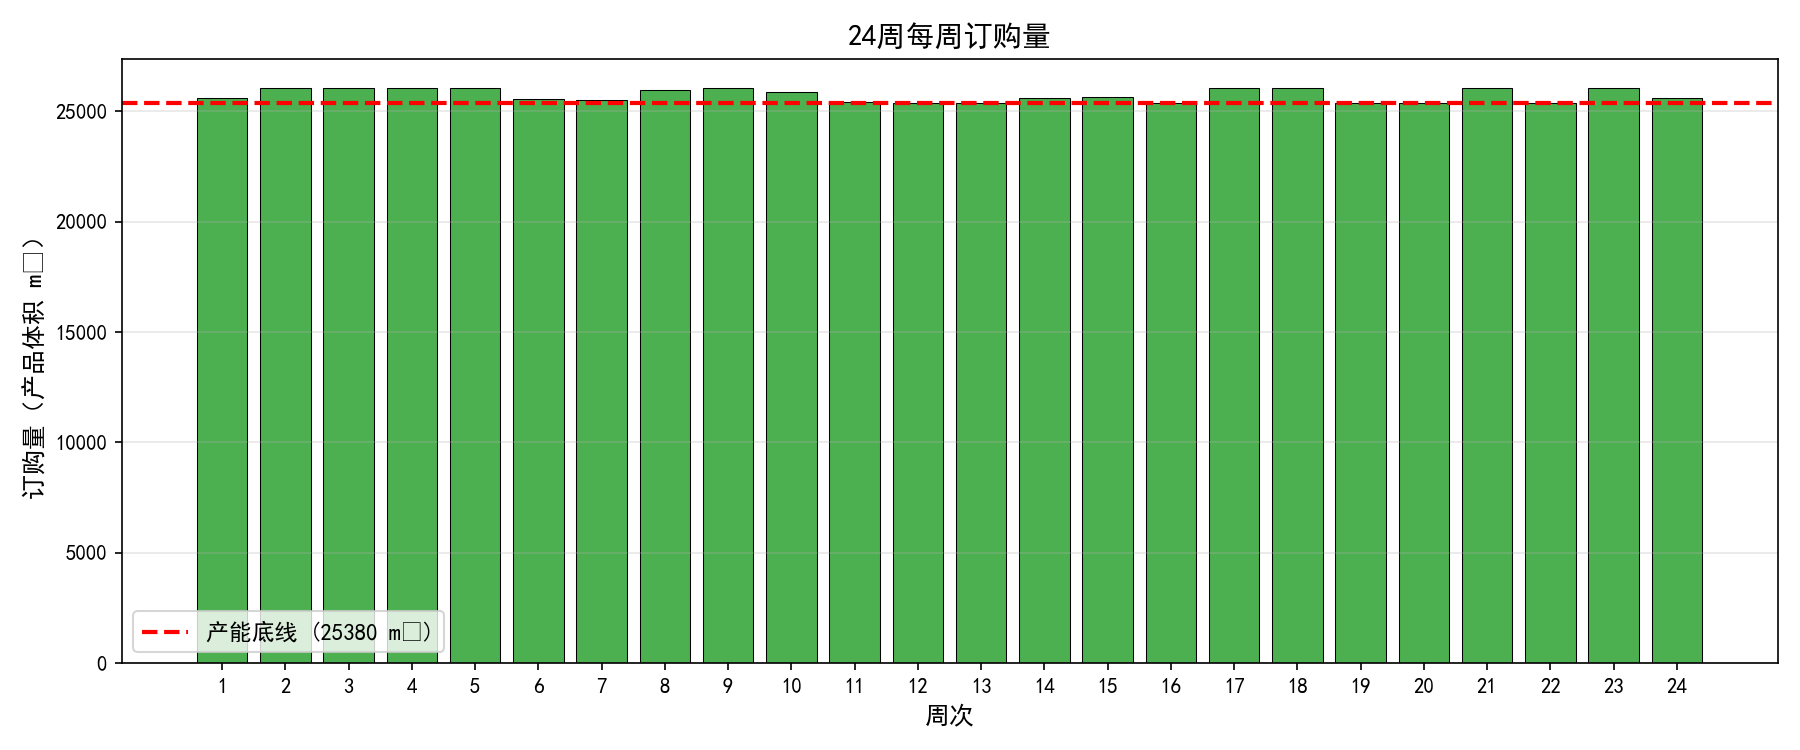
\includegraphics[width=0.8\textwidth]{problem2_weekly_volume.png}
\caption{24周订购量柱状图}
\label{fig:volume}
\end{figure}
24周订购量均高于百分之九十产能底线25380立方米，最低周为25381立方米，紧贴约束边界。

图\ref{fig:suppliers}展示了每周各类供应商的数量分布。
\begin{figure}[H]
\centering
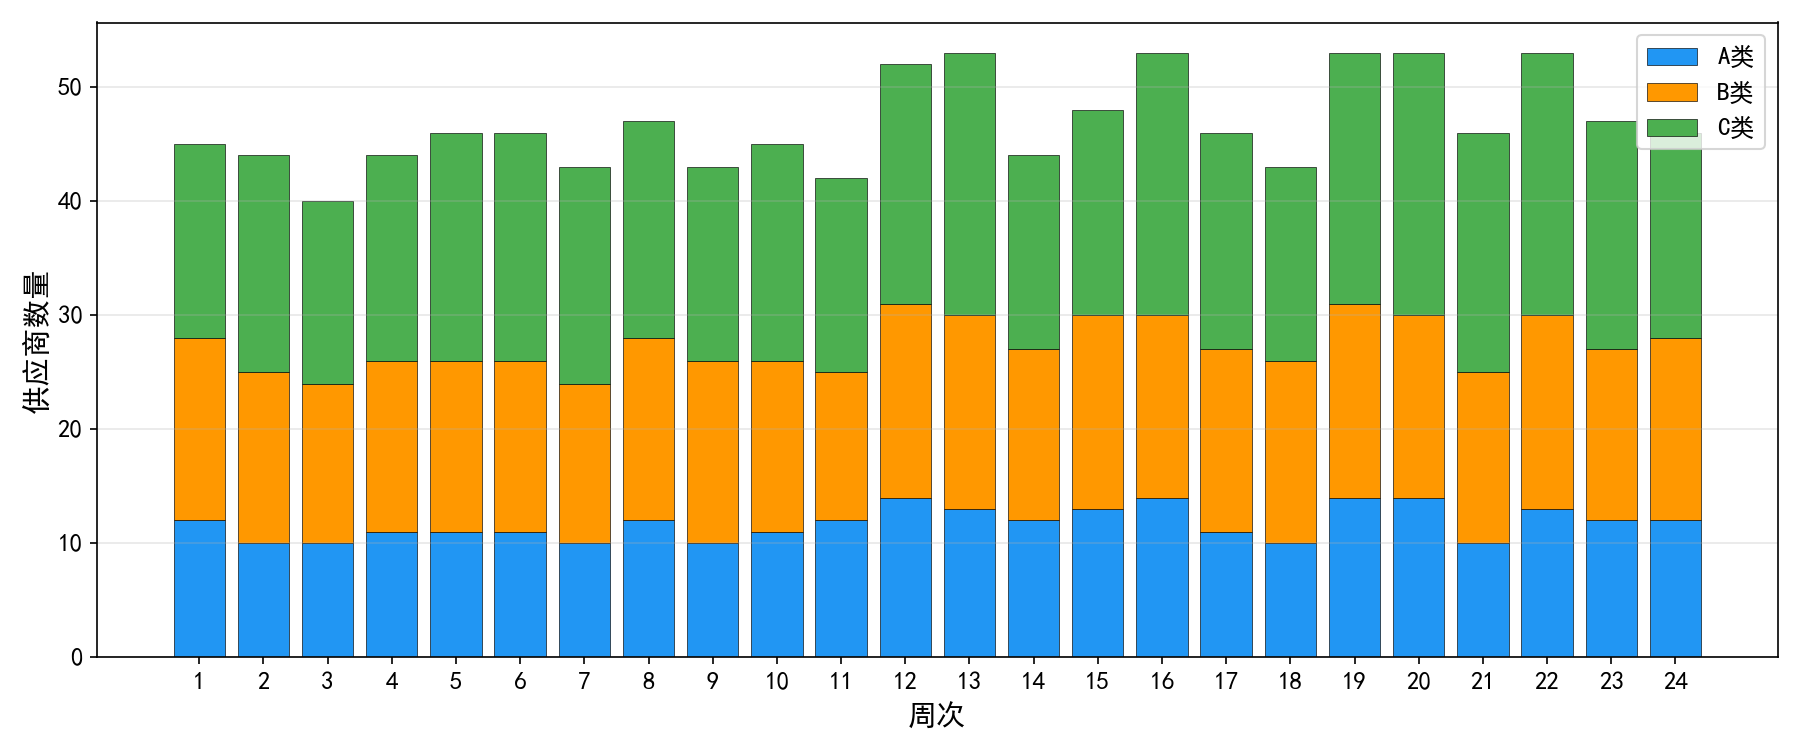
\includegraphics[width=0.8\textwidth]{problem2_weekly_suppliers.png}
\caption{每周供应商数量堆叠图}
\label{fig:suppliers}
\end{figure}
A类每周10至14家，B类13至17家，C类16至23家，三类材料每周均有充分覆盖。

图\ref{fig:heatmap}展示了55家供应商在24周的订购情况。
\begin{figure}[H]
\centering
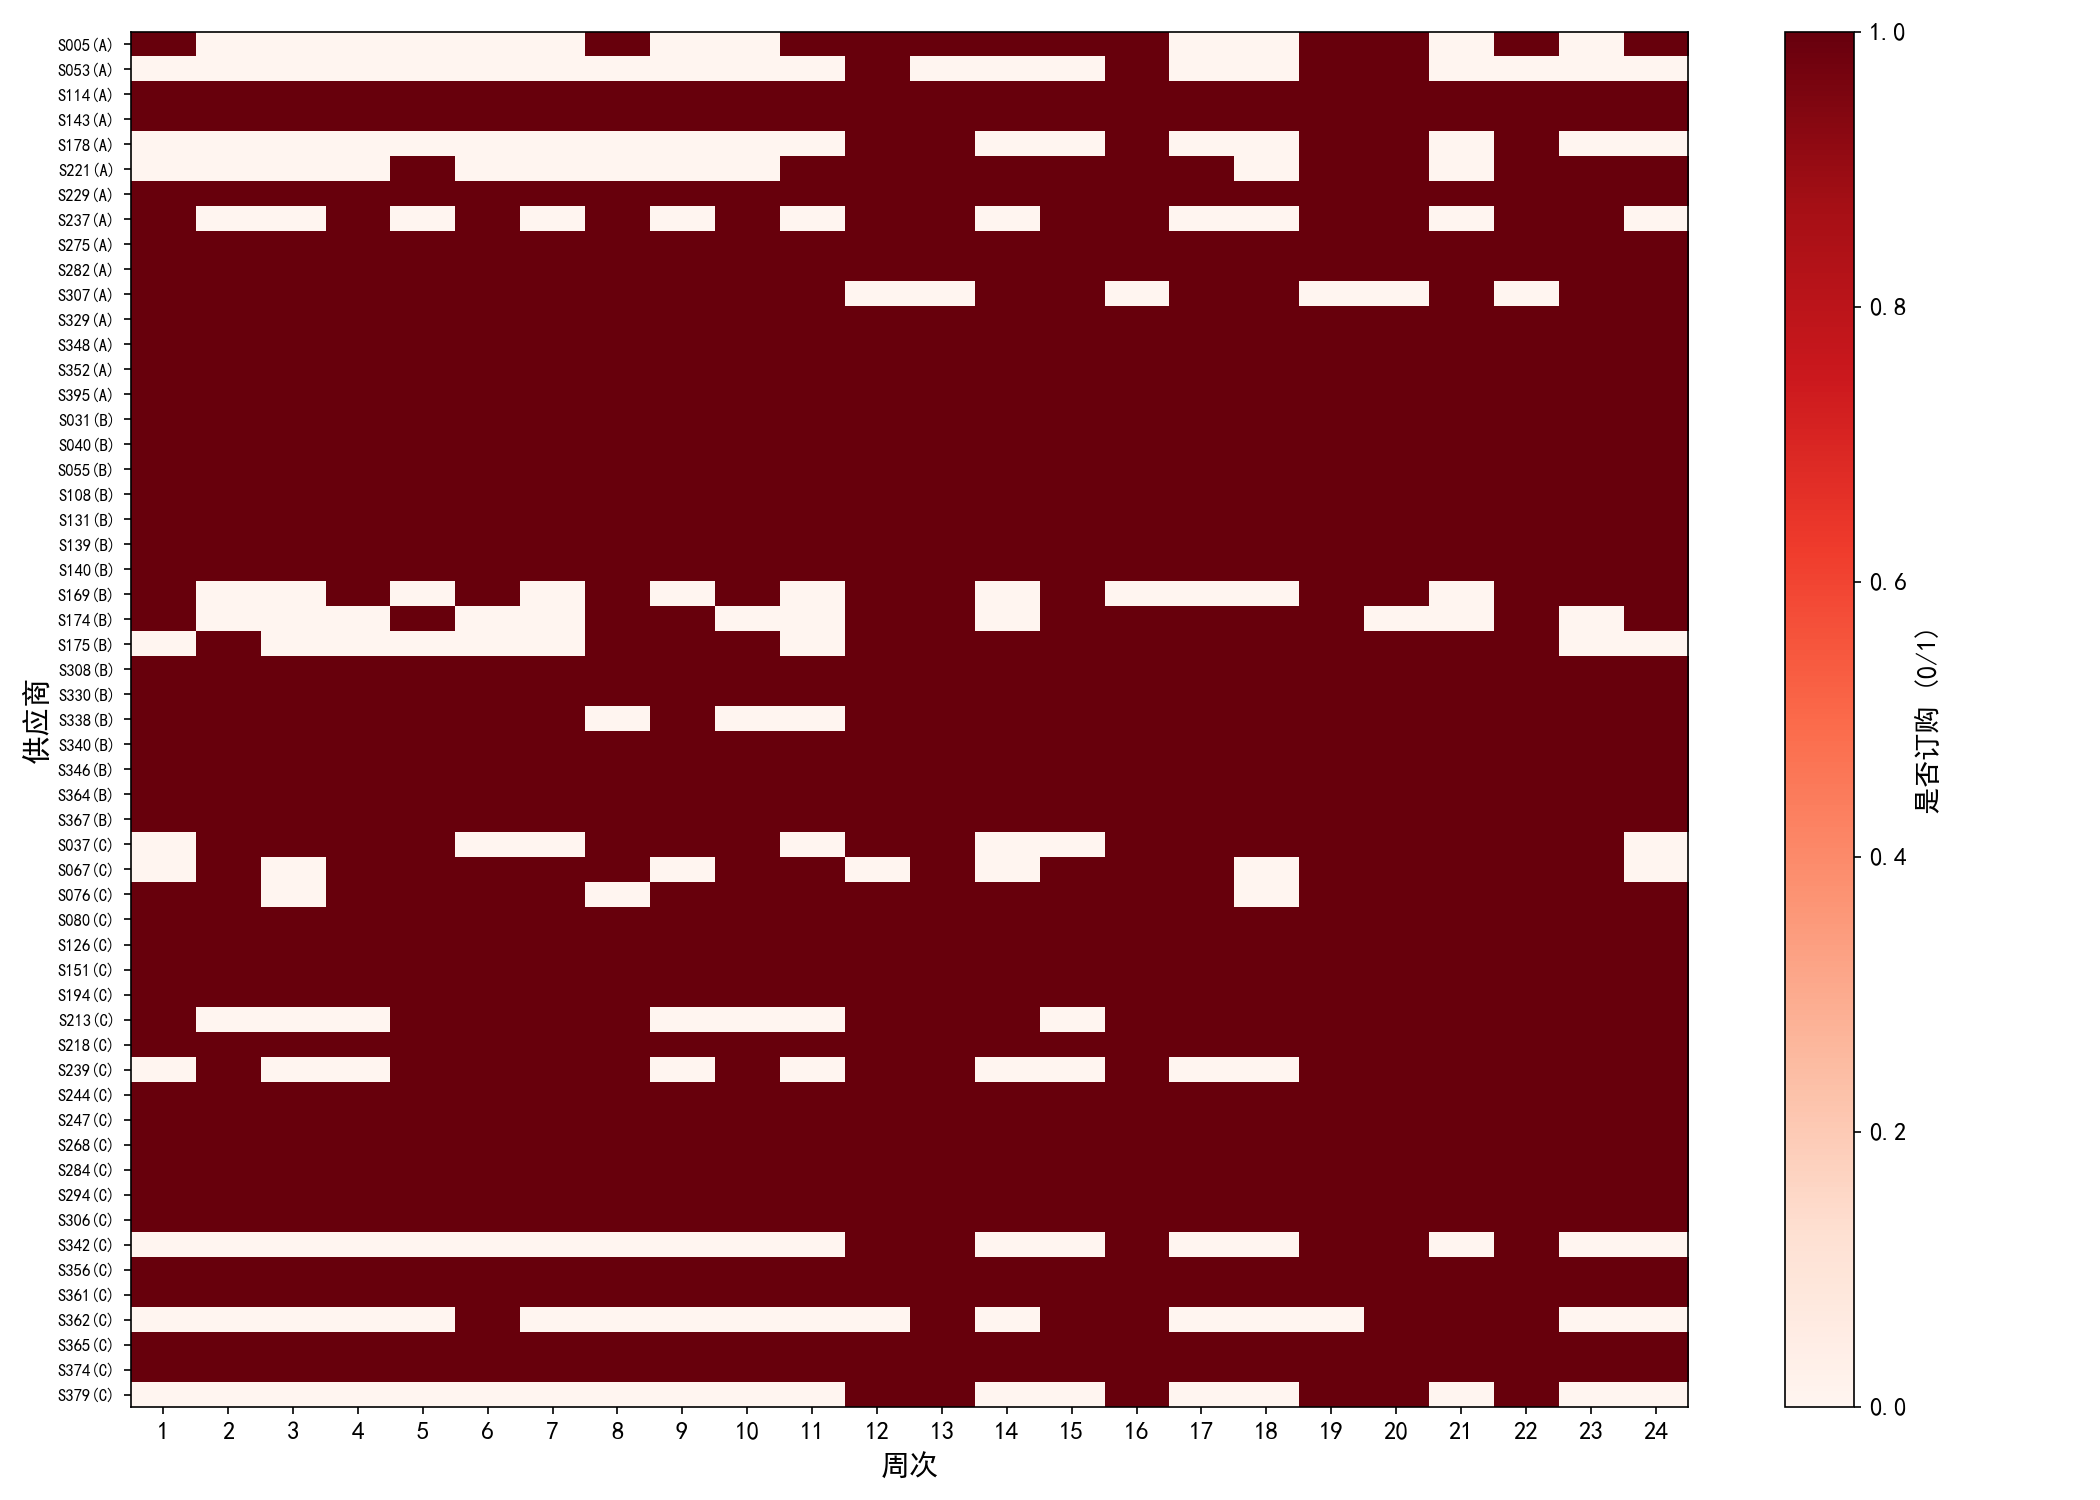
\includegraphics[width=0.85\textwidth]{problem2_heatmap.png}
\caption{供应商周次订购热力图}
\label{fig:heatmap}
\end{figure}
行为55家供应商按材料类型分组，列为24周。深色表示该周向该供应商订货。部分供应商$K_i=24$每周必选，属于高频次约束的必选供应商；部分供应商$K_i$较小，调度弹性较强，模型通过调节这些供应商的排班实现成本微优化。

\subsubsection{结果分析与验证}

\textbf{紧约束特征：}最低周仅超出产能底线1立方米，55家全选时的周产能为26176立方米，仅为底线要求的百分之103.1，产能余量仅796立方米。平均每周选中46.8家，仅8家轮休。说明问题二本质上不是从55家中宽裕地挑选子集，而是每周仅能少用少数几家的极限调度问题。

\textbf{成本结构：}A类与C类单位产品成本均为0.720，模型在两类间无偏好，最优解在A/C排班上存在等价替换空间。B类单位成本为0.726，高出0.83%，模型有极微弱的惩罚倾向，但在紧约束下该偏好几乎不影响实际排班。

\textbf{频次分布：}频次约束总和为1081次，上限为1320次，平均每家供应商需订货约19.6次。部分供应商$K_i=24$为必选，其订购量固定；真正具有调度弹性的为$K_i$较小的供应商，优化空间主要体现在这些供应商的排班选择上。

\subsection{问题三模型建立及求解}

\subsubsection{模型建立}

对每家供应商定义有效周上的供货偏差：
\begin{equation}
D_{ij} = S_{ij} - O_{ij}, \quad j \in W_i
\label{eq:deviation}
\end{equation}
$D_{ij} > 0$表示超额供货，$D_{ij} < 0$表示缺货。对偏差序列执行ADF单位根检验，若不平稳则差分至平稳。再使用Ljung-Box检验判断残差是否存在自相关。若序列平稳且存在显著自相关，拟合ARIMA($p,d,q$)模型：
\begin{equation}
\phi(B)(1-B)^d D_t = \theta(B)\varepsilon_t
\label{eq:arima}
\end{equation}
其中$\phi(B)=1-\phi_1B-\cdots-\phi_pB^p$为自回归多项式，$\theta(B)=1-\theta_1B-\cdots-\theta_qB^q$为移动平均多项式，$B$为滞后算子，$d$为差分阶数。若序列为白噪声，则使用样本均值作为预测值：
\begin{equation}
\hat{D}_{i} = \frac{1}{N_i} \sum_{j \in W_i} D_{ij}
\label{eq:mean}
\end{equation}

外推未来24周偏差预测值$\hat{D}_{ij}$，叠加固定订货量得到实际供货预测：
\begin{equation}
\hat{S}_{ij} = (Q_i + \hat{D}_{ij}) \cdot x_{ij}
\label{eq:pred_supply}
\end{equation}
其中$x_{ij}$为问题二的订货决策结果。再按材料消耗率折算为周产品体积：
\begin{equation}
\hat{T}_j = \sum_{i=1}^{55} \frac{\hat{S}_{ij}}{u_i}
\label{eq:total_volume}
\end{equation}
每周的产能满足率计算如下：
\begin{equation}
\text{满足率}_j = \frac{\hat{T}_j}{28200} \times 100\%
\label{eq:fulfillment_rate}
\end{equation}
将各周计算结果取整后统计达标周数与比例。

\subsubsection{模型求解}

模型选择结果如图\ref{fig:model_dist}所示。

\begin{figure}[H]
\centering
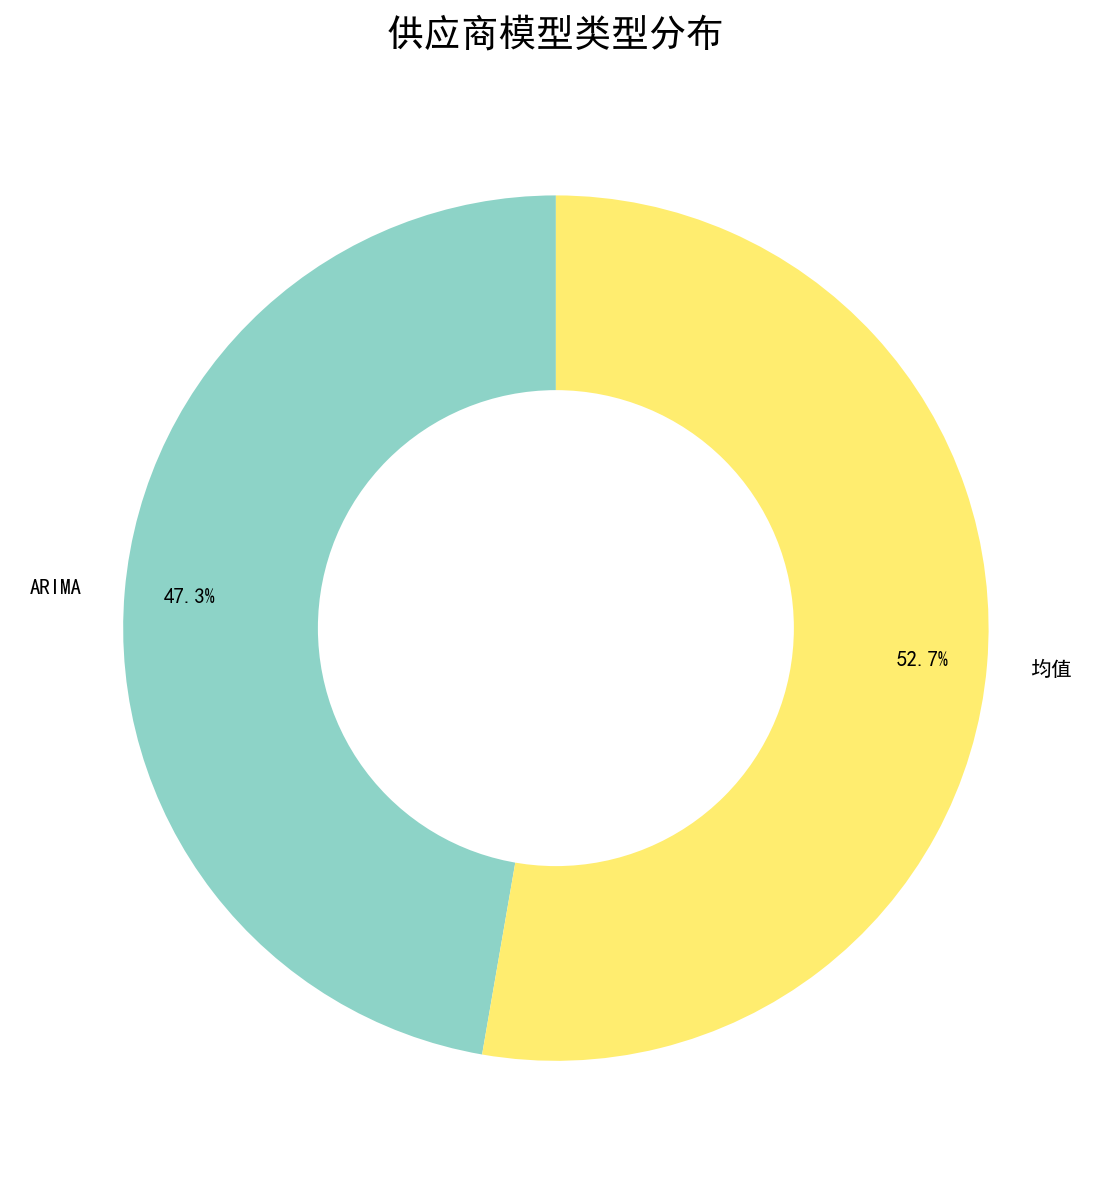
\includegraphics[width=0.7\textwidth]{problem3E_model_distribution.png}
\caption{模型类型分布饼图}
\label{fig:model_dist}
\end{figure}
百分之47.3的供应商偏差序列存在显著自相关，使用ARIMA模型；百分之52.7的供应商偏差序列为白噪声，使用均值模型。约半数供应商的偏差具有时间记忆性。

图\ref{fig:gap_dist}展示了55家供应商的平均偏差分布。

\begin{figure}[H]
\centering
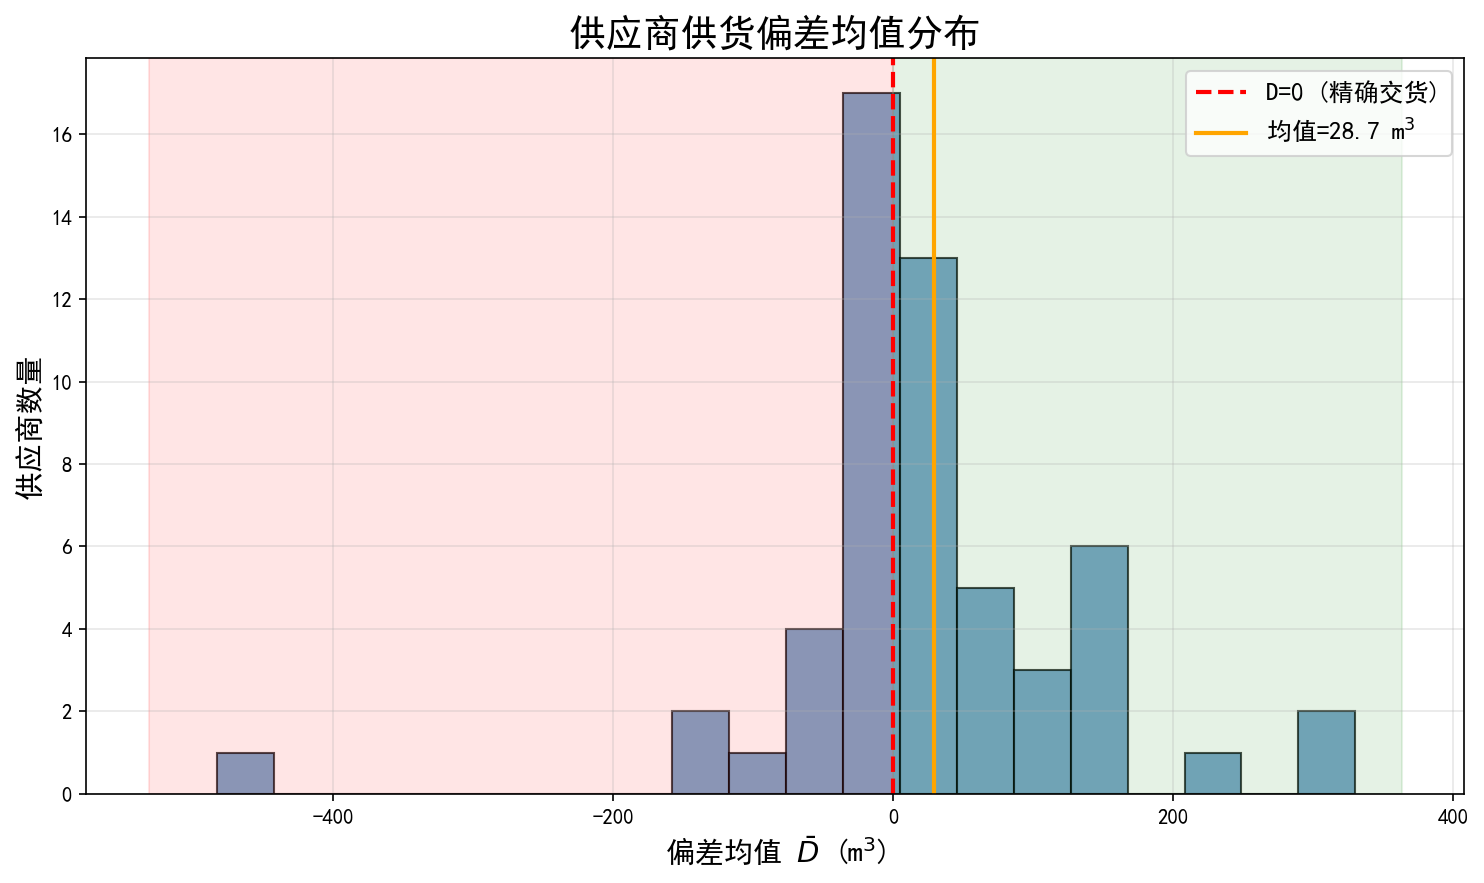
\includegraphics[width=0.7\textwidth]{problem3E_gap_distribution.png}
\caption{供应商平均偏差分布直方图}
\label{fig:gap_dist}
\end{figure}
百分之80的供应商平均偏差为正，即平均供货量超过订货量，平均超额28.66立方米，反映了供应商整体超额供货的历史特征。

图\ref{fig:acf}展示了一家典型供应商的偏差序列自相关函数图。

\begin{figure}[H]
\centering
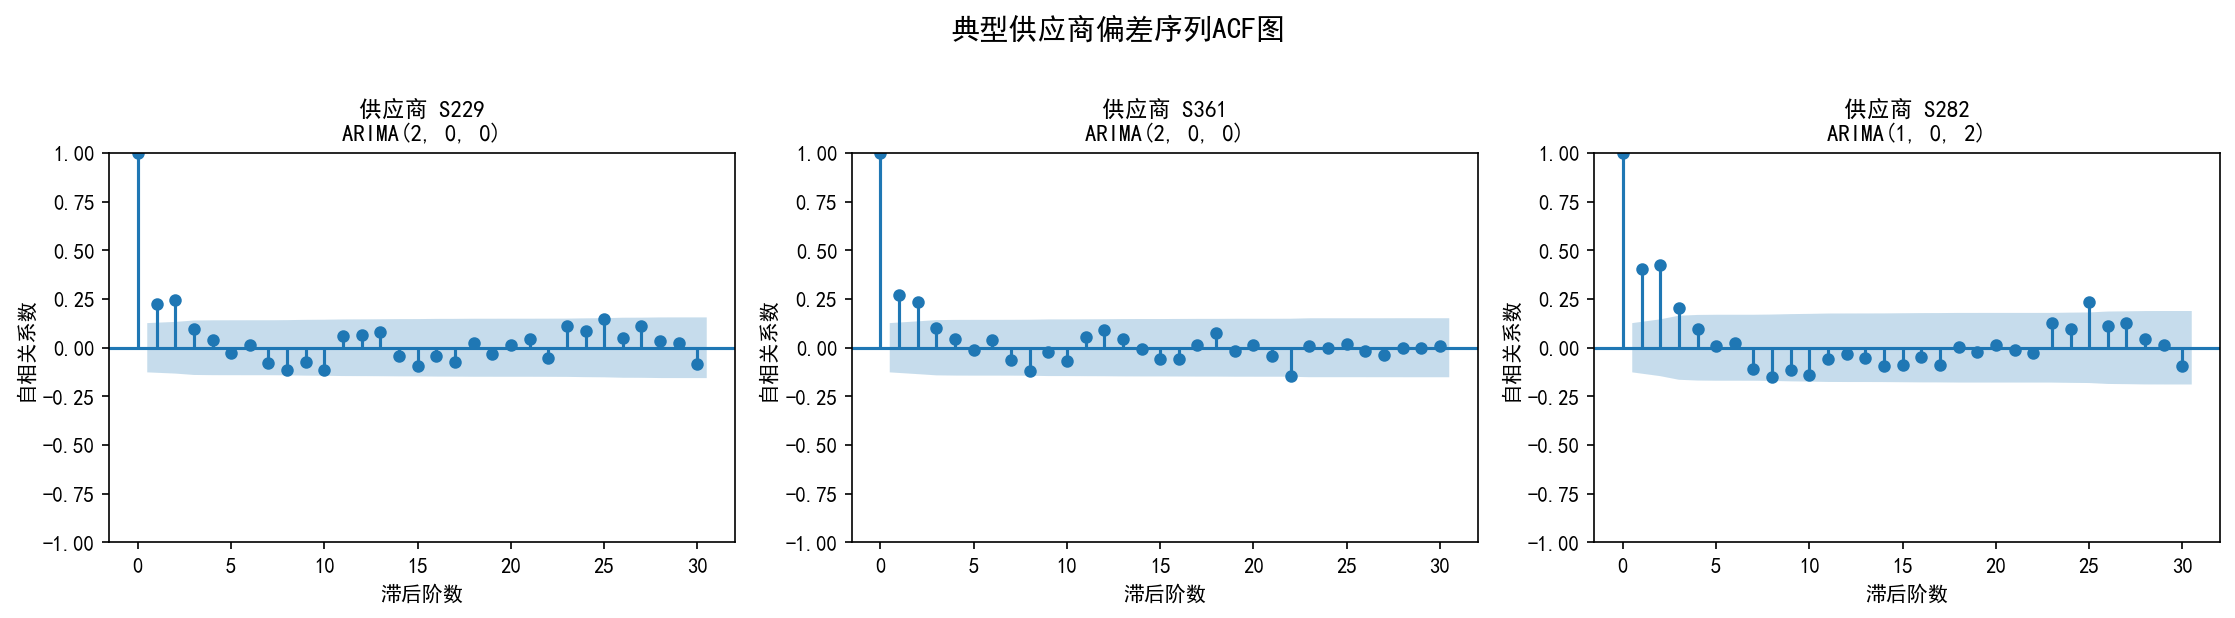
\includegraphics[width=0.8\textwidth]{problem3E_acf_example.png}
\caption{偏差序列自相关函数图}
\label{fig:acf}
\end{figure}
部分供应商偏差具有二阶自回归结构，即前两周的偏差值对当前偏差有显著影响，ARIMA模型可以捕捉这种时间惯性。

图\ref{fig:weekly_supply}展示了未来24周的周供应量预测结果。

\begin{figure}[H]
\centering
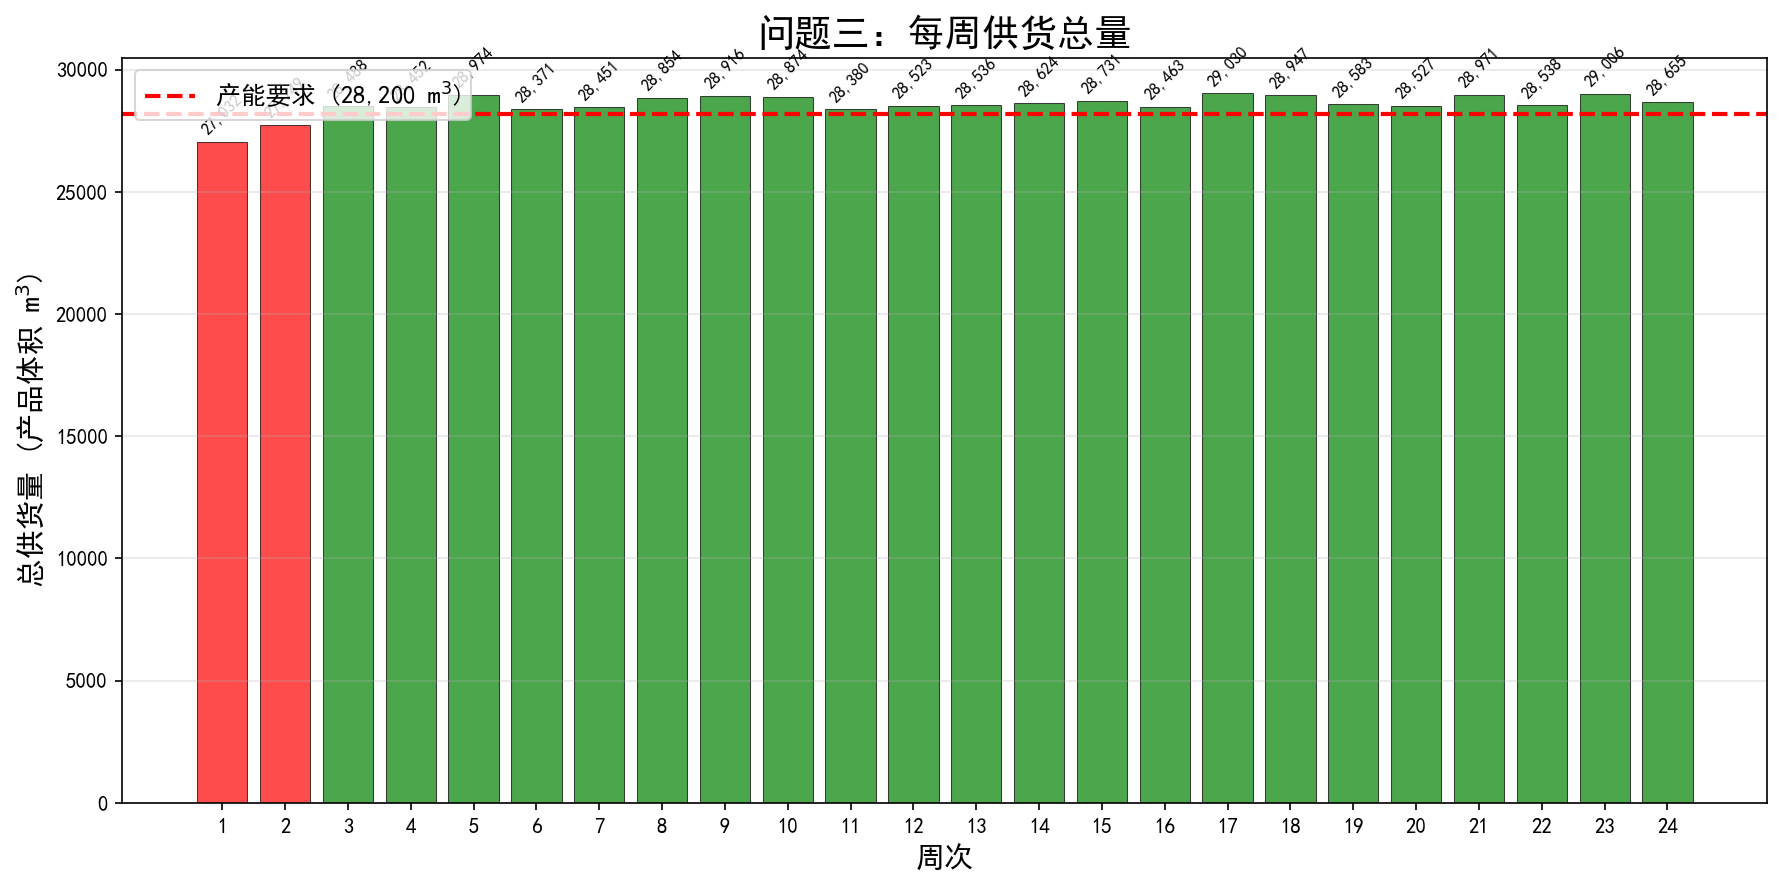
\includegraphics[width=0.8\textwidth]{problem3E_weekly_supply.png}
\caption{24周供应量预测柱状图}
\label{fig:weekly_supply}
\end{figure}
24周中有22周达到满产能需求，达标比例百分之91.7。第1周和第2周因模型启动初期偏差积累不足，预测精度略低于成熟期。

图\ref{fig:fulfillment}展示了每周的产能满足率。

\begin{figure}[H]
\centering
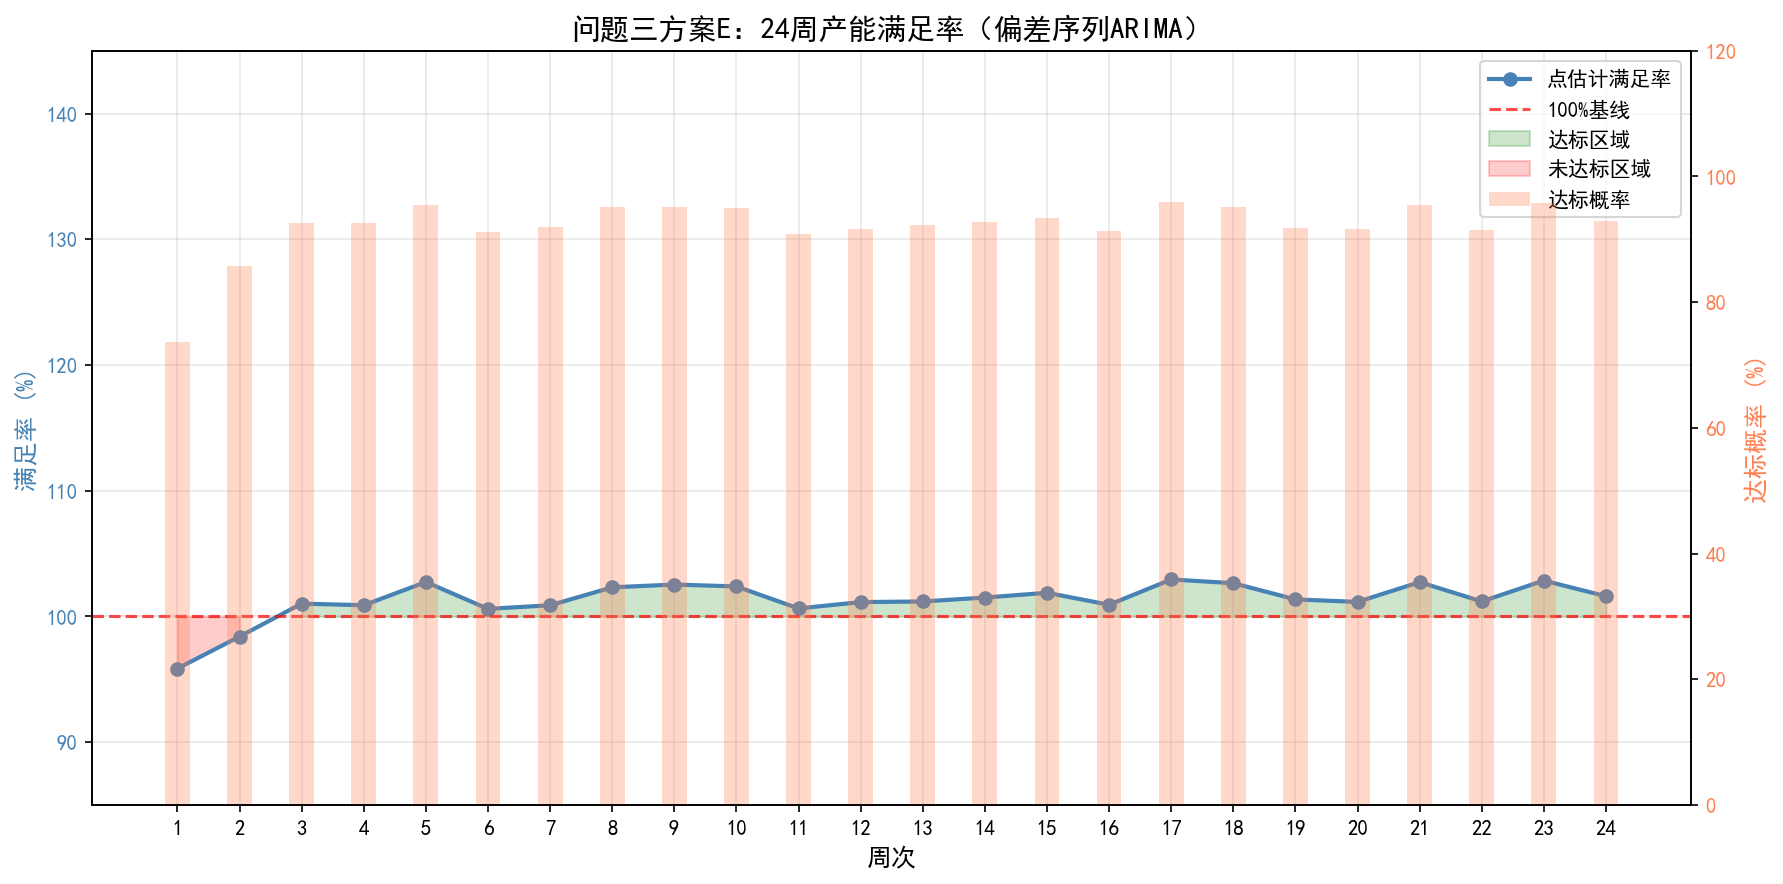
\includegraphics[width=0.7\textwidth]{problem3E_fulfillment_rate.png}
\caption{每周产能满足率柱状图}
\label{fig:fulfillment}
\end{figure}
平均满足率为百分之101.31，未达标的第1周和第2周满足率分别为百分之95.86和百分之98.40，缺口在百分之2至百分之4之间。

\subsubsection{结果展示}

\begin{table}[H]
\centering
\caption{问题三产能满足率输出结果}
\label{tab:fulfillment}
\zihao{5}
\begin{tabular}{cc}
\toprule
指标 & 数值 \\
\midrule
平均满足率 & 101.31\% \\
最小满足率 & 95.86\% \\
最大满足率 & 102.94\% \\
达标周数 & 22周 \\
达标比例 & 91.7\% \\
平均达标概率 & 92.12\% \\
\bottomrule
\end{tabular}
\end{table}
点估计给出22周达标，蒙特卡洛模拟给出每周约百分之92的达标概率，两者高度一致。

\subsubsection{结果分析与验证}

以第1至216周为训练期、第217至240周为测试期进行回测。图\ref{fig:backtest_weekly}展示了测试期24周真实总量与模型预测总量的逐周对比。

\begin{figure}[H]
\centering
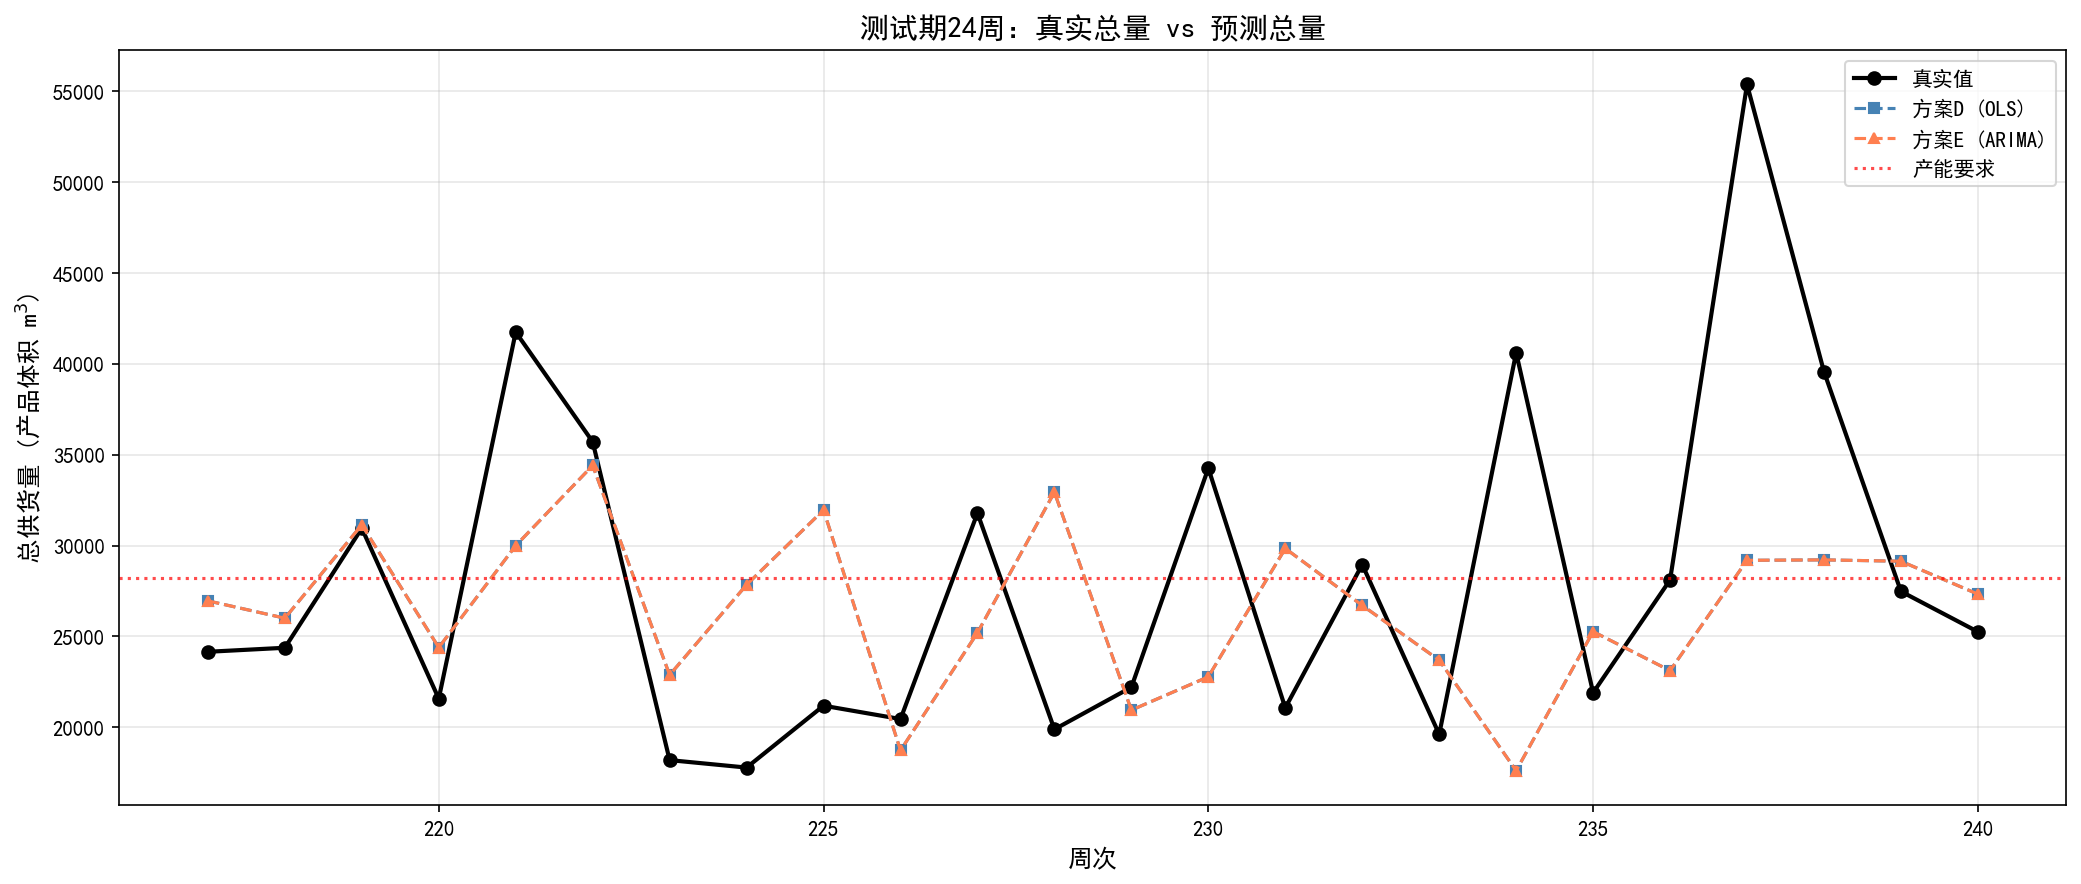
\includegraphics[width=0.5\textwidth]{problem3_backtest_weekly.png}
\caption{回测期周供应量对比折线图}
\label{fig:backtest_weekly}
\end{figure}
蓝色实线为真实供应量，橙色虚线为偏差ARIMA预测值，绿色虚线为池化OLS预测值。偏差ARIMA预测曲线更贴近真实曲线。

图\ref{fig:backtest_scatter}展示了逐观测预测值与真实值的散点对比。

\begin{figure}[H]
\centering
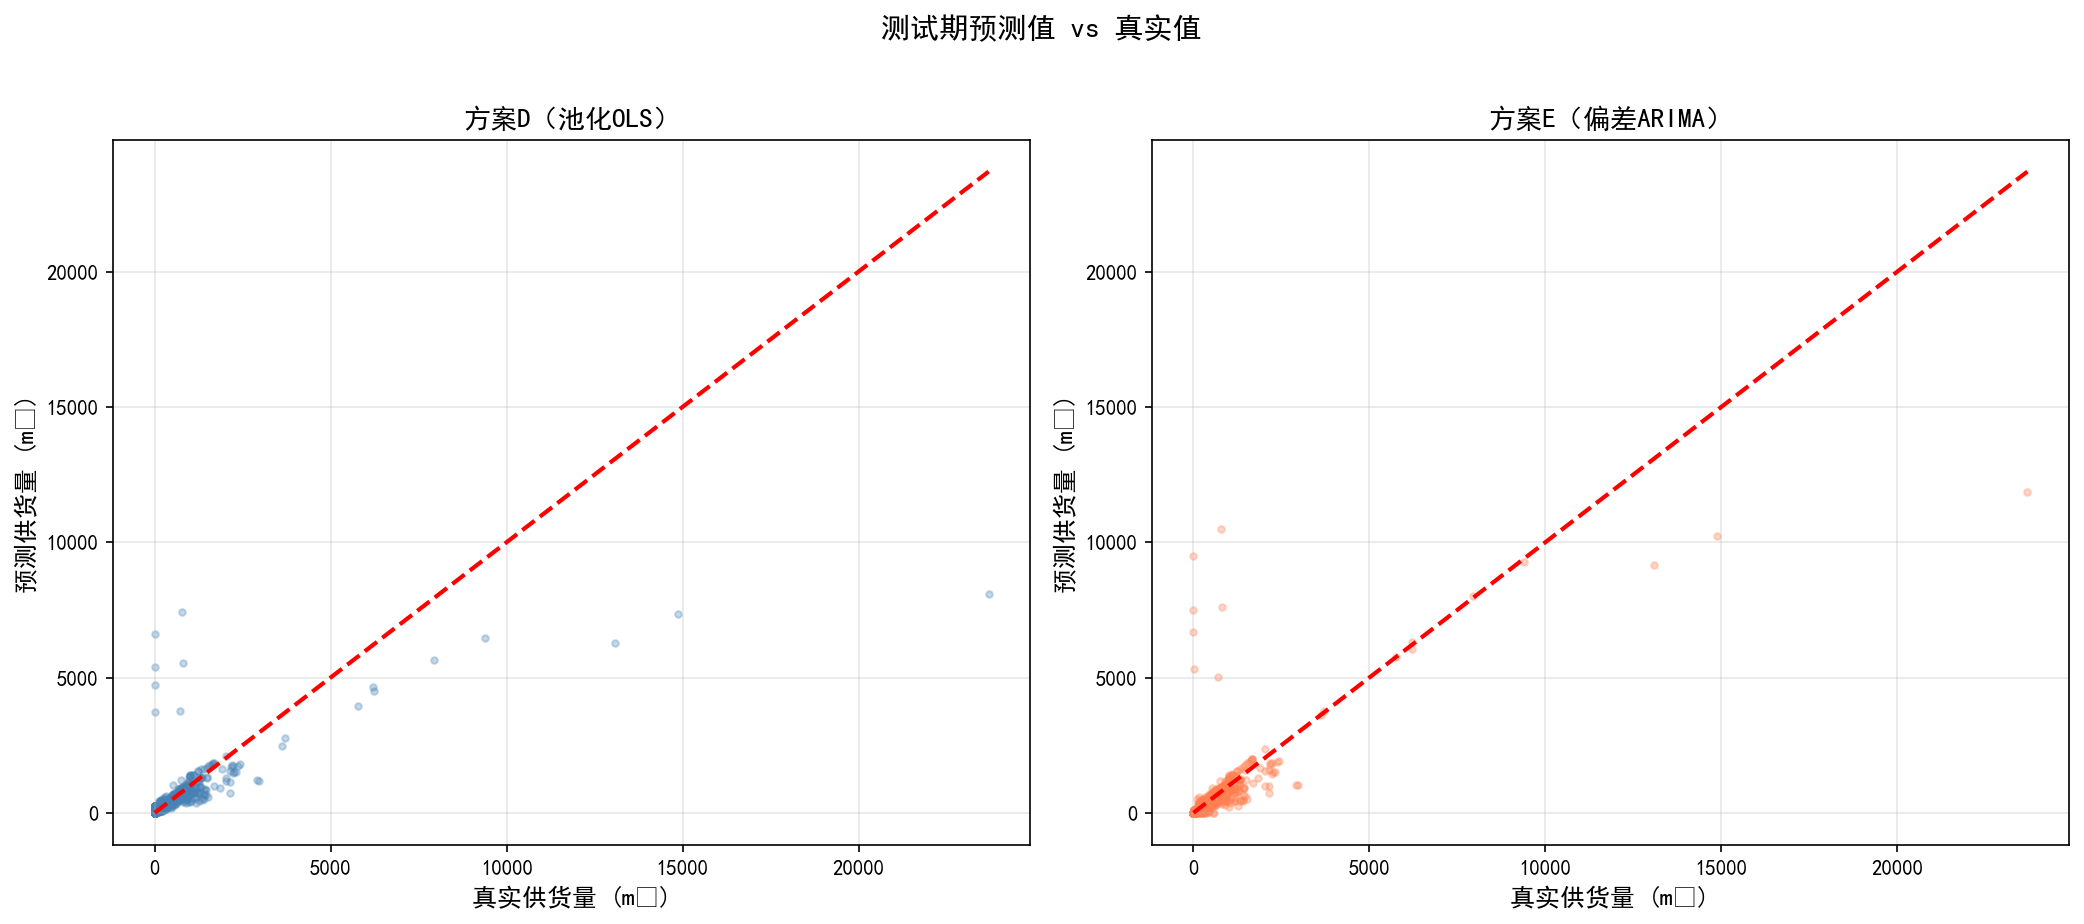
\includegraphics[width=0.7\textwidth]{problem3_backtest_scatter.png}
\caption{回测预测值与真实值散点图}
\label{fig:backtest_scatter}
\end{figure}
越接近对角线表示预测越准确。偏差ARIMA的点分布更集中在对角线附近，说明其预测精度更高。偏差ARIMA的均方根误差和平均绝对误差分别比池化线性回归低百分之9.87和百分之7.21，决定系数提升6.8个百分点，验证了模型选择的合理性。


\section{模型的评价与推广}

\subsection{模型的优点}

\begin{enumerate}[label=\arabic*.]
  \item CRITIC法赋予供货达标率最高权重0.5325，成功剔除量大但履约差的伪优质供应商，避免熵权法因值域跨度大导致的权重分配失衡。
  \item 0-1整数规划模型在55家供应商全选产能余量仅3.1\%的约束下秒级求得全局最优解，所有周次订购量贴近25380立方米且最小超量仅1立方米，验证了模型处理高维离散组合优化问题的精确性。
  \item 直接对“供货-订货”偏差建立ARIMA模型，有效规避了小订单场景下供货率比值失真的系统性误差。
\end{enumerate}

\subsection{模型的缺点}

\begin{enumerate}[label=\arabic*.]
  \item 问题一未对有效观测周数设置下限阈值，少数供应商的特征估计存在不确定性。
  \item 问题三假设供应商的供货行为模式在未来保持不变，若发生结构性变化，历史偏差将不再适用。
\end{enumerate}

\subsection{模型的推广}

本模型可推广至其他制造企业的供应链管理。对于问题一的评价模型，可根据企业实际需求调整特征指标。对于问题三的预测模型，可引入外部变量如原材料价格、季节因素等，提高预测精度。


% ======================== 参考文献 ========================
\begin{thebibliography}{99}
\addcontentsline{toc}{section}{参考文献}

\bibitem{ref1} Diakoulaki D, Mavrotas G, Papayannakis L. Determining objective weights in multiple criteria problems: The CRITIC method[J]. Computers \& Operations Research, 1995, 22(7): 763-770.

\bibitem{ref2} Hwang C L, Yoon K. Multiple Attribute Decision Making: Methods and Applications[M]. New York: Springer-Verlag, 1981.

\bibitem{ref3} Box G E P, Jenkins G M. Time Series Analysis: Forecasting and Control[M]. Revised ed. San Francisco: Holden-Day, 1976.

\bibitem{ref4} Xie Z, Tian G, Tao Y. A Multi-Criteria Decision-Making Framework for Sustainable Supplier Selection in the Circular Economy and Industry 4.0 Era[J]. Sustainability, 2022, 14(24): 16809.

\bibitem{ref5} Luo J, Wang Y, Liu C, et al. Data-driven optimization strategy of raw material procurement under uncertainties of price fluctuations and production demand[J]. Computers \& Industrial Engineering, 2025, 208: 111425.

\bibitem{ref6} 高洁, 文琼瑶, 明思扬, 等. 基于评价体系与最优化的原材料订购和运输问题研究[J]. 运筹与模糊学, 2023, 13(1): 129-138.

\bibitem{ref7} DeepSeek. DeepSeek V4 Pro 大语言模型[EB/OL]. 2026.

\bibitem{ref8} 阿里巴巴云计算. 通义千问 Qwen 3.7 Max 大语言模型[EB/OL]. 2026.

\end{thebibliography}


% ======================== 附录 ========================
\newpage
\appendix
\renewcommand{\thesection}{附录 \Alph{section}}
\renewcommand{\thesubsection}{\Alph{section}.\arabic{subsection}}
\renewcommand{\thesubsubsection}{\Alph{section}.\arabic{subsection}.\arabic{subsubsection}}
\titleformat{\section}
  {\centering\heiti\zihao{-3}\bfseries}
  {\thesection}{1em}{}

\section{支撑文件列表}

\begin{table}[H]
\centering
\zihao{5}
\begin{tabular}{ll}
\toprule
文件名 & 说明 \\
\midrule
\multicolumn{2}{l}{\textbf{Python代码}} \\
problem1\_main.py & 问题一主程序 \\
problem\_data\_loader.py & 数据加载模块 \\
problem\_indicators.py & 特征指标计算模块 \\
problem\_normalize.py & 数据标准化模块 \\
problem\_critic\_weight.py & CRITIC权重计算模块 \\
problem\_topsis.py & TOPSIS排序模块 \\
problem\_ordering\_solver.py & 0-1整数规划求解器 \\
problem2\_main.py & 问题二主程序 \\
problem3\_predictor.py & ARIMA偏差预测器 \\
problem3\_main.py & 问题三主程序 \\
problem3\_backtest.py & 回测验证模块 \\
\midrule
\multicolumn{2}{l}{\textbf{结果数据}} \\
problem1\_supplier\_ranking.csv & 402家供应商完整排名 \\
problem1\_top55.csv & 前55家供应商子集 \\
problem3\_weekly\_summary.csv & 每周供应汇总 \\
problem3\_capacity\_stats.csv & 产能输出统计 \\
附件A 订购方案数据结果+队号.xlsx & 问题二订购方案与问题三供应方案 \\
\midrule
\multicolumn{2}{l}{\textbf{说明文档}} \\
AI工具使用说明.pdf & AI工具使用说明 \\
\bottomrule
\end{tabular}
\end{table}



\section{相关代码}

\codefile{problem1\_main.py}{问题一主程序}{./code/problem1_main.py}

\codefile{problem\_data\_loader.py}{数据加载模块}{./code/problem_data_loader.py}

\codefile{problem\_indicators.py}{特征指标计算模块}{./code/problem_indicators.py}

\codefile{problem\_normalize.py}{数据标准化模块}{./code/problem_normalize.py}

\codefile{problem\_critic\_weight.py}{CRITIC权重计算模块}{./code/problem_critic_weight.py}

\codefile{problem\_topsis.py}{TOPSIS排序模块}{./code/problem_topsis.py}

\codefile{problem\_ordering\_solver.py}{0-1整数规划求解器}{./code/problem_ordering_solver.py}

\codefile{problem2\_main.py}{问题二主程序}{./code/problem2_main.py}

\codefile{problem3\_predictor.py}{ARIMA偏差预测器}{./code/problem3_predictor.py}

\codefile{problem3\_main.py}{问题三主程序}{./code/problem3_main.py}

\codefile{problem3\_backtest.py}{回测验证模块}{./code/problem3_backtest.py}


\end{document}
